% Options for packages loaded elsewhere
\PassOptionsToPackage{unicode}{hyperref}
\PassOptionsToPackage{hyphens}{url}
%
\documentclass[
  12pt,
  a4j]{ltjarticle}
\usepackage{amsmath,amssymb}
\usepackage{lmodern}
\usepackage{iftex}
\ifPDFTeX
  \usepackage[T1]{fontenc}
  \usepackage[utf8]{inputenc}
  \usepackage{textcomp} % provide euro and other symbols
\else % if luatex or xetex
  \usepackage{unicode-math}
  \defaultfontfeatures{Scale=MatchLowercase}
  \defaultfontfeatures[\rmfamily]{Ligatures=TeX,Scale=1}
\fi
% Use upquote if available, for straight quotes in verbatim environments
\IfFileExists{upquote.sty}{\usepackage{upquote}}{}
\IfFileExists{microtype.sty}{% use microtype if available
  \usepackage[]{microtype}
  \UseMicrotypeSet[protrusion]{basicmath} % disable protrusion for tt fonts
}{}
\makeatletter
\@ifundefined{KOMAClassName}{% if non-KOMA class
  \IfFileExists{parskip.sty}{%
    \usepackage{parskip}
  }{% else
    \setlength{\parindent}{0pt}
    \setlength{\parskip}{6pt plus 2pt minus 1pt}}
}{% if KOMA class
  \KOMAoptions{parskip=half}}
\makeatother
\usepackage{xcolor}
\IfFileExists{xurl.sty}{\usepackage{xurl}}{} % add URL line breaks if available
\IfFileExists{bookmark.sty}{\usepackage{bookmark}}{\usepackage{hyperref}}
\hypersetup{
  pdftitle={Buffered I/Oの速度の計測と考察},
  pdfauthor={205723K 佐野巧曜},
  hidelinks,
  pdfcreator={LaTeX via pandoc}}
\urlstyle{same} % disable monospaced font for URLs
\usepackage[margin=1in]{geometry}
\usepackage{listings}
\newcommand{\passthrough}[1]{#1}
\lstset{defaultdialect=[5.3]Lua}
\lstset{defaultdialect=[x86masm]Assembler}
\usepackage{longtable,booktabs,array}
\usepackage{calc} % for calculating minipage widths
% Correct order of tables after \paragraph or \subparagraph
\usepackage{etoolbox}
\makeatletter
\patchcmd\longtable{\par}{\if@noskipsec\mbox{}\fi\par}{}{}
\makeatother
% Allow footnotes in longtable head/foot
\IfFileExists{footnotehyper.sty}{\usepackage{footnotehyper}}{\usepackage{footnote}}
\makesavenoteenv{longtable}
\usepackage{graphicx}
\makeatletter
\def\maxwidth{\ifdim\Gin@nat@width>\linewidth\linewidth\else\Gin@nat@width\fi}
\def\maxheight{\ifdim\Gin@nat@height>\textheight\textheight\else\Gin@nat@height\fi}
\makeatother
% Scale images if necessary, so that they will not overflow the page
% margins by default, and it is still possible to overwrite the defaults
% using explicit options in \includegraphics[width, height, ...]{}
\setkeys{Gin}{width=\maxwidth,height=\maxheight,keepaspectratio}
% Set default figure placement to htbp
\makeatletter
\def\fps@figure{htbp}
\makeatother
\setlength{\emergencystretch}{3em} % prevent overfull lines
\providecommand{\tightlist}{%
  \setlength{\itemsep}{0pt}\setlength{\parskip}{0pt}}
\setcounter{secnumdepth}{-\maxdimen} % remove section numbering
% adjust the position of an image to be displayed
\usepackage{float}
\let\origfigure\figure
\let\endorigfigure\endfigure
\renewenvironment{figure}[1][2] {
    \expandafter\origfigure\expandafter[H]
} {
    \endorigfigure
}

% add frame to a coding block
\usepackage{listings}
\lstset{
    numbers=left,
    frame=single,
    tabsize=2,
    breaklines=true,
}

% centre the title
\usepackage{titling}
\renewcommand{\maketitlehooka}{\null\mbox{}\vfill}
\renewcommand{\maketitlehookd}{\vfill\null}
\ifLuaTeX
  \usepackage{selnolig}  % disable illegal ligatures
\fi

\title{Buffered I/Oの速度の計測と考察}
\author{205723K 佐野巧曜}
\date{2023年 1月 8日}

\begin{document}
\maketitle

\hypertarget{ux5b9fux9a13ux30c7ux30fcux30bf}{%
\section{実験データ}\label{ux5b9fux9a13ux30c7ux30fcux30bf}}

GolangのbufioパッケージでBuffered I/Oを実装した。

実験の計測したときの環境は以下の通りである。

\begin{lstlisting}
Operating System: Ubuntu 22.04.1 LTS
          Kernel: Linux 5.15.0-53-generic
    Architecture: x86-64
 Hardware Vendor: Dell Inc.
  Hardware Model: PowerEdge R740
     File System: ext4
      Go version: go1.19.1 linux/amd64
\end{lstlisting}

以下の2つのグラフがバッファなしから16384
bytesまでのバッファでファイルに書き出したときの速度のグラフである。

横軸がファイルサイズ(bytes)で縦軸が実行時間(ナノ秒)である

\begin{figure}
\centering
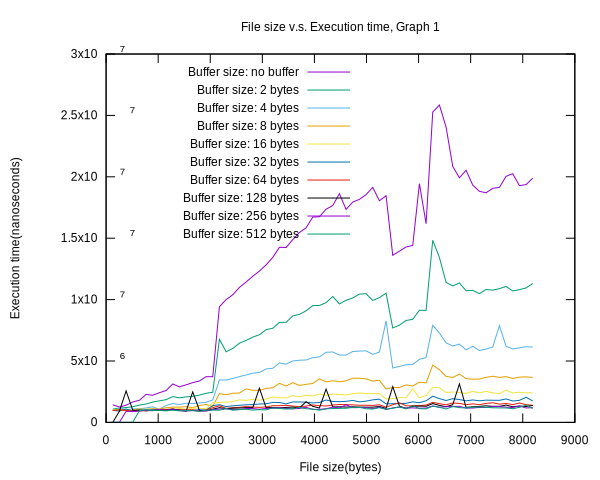
\includegraphics{../png/graph1.png}
\caption{512 bytes以内範囲のバッファの書き出しの速度のグラフ}
\end{figure}

\begin{figure}
\centering
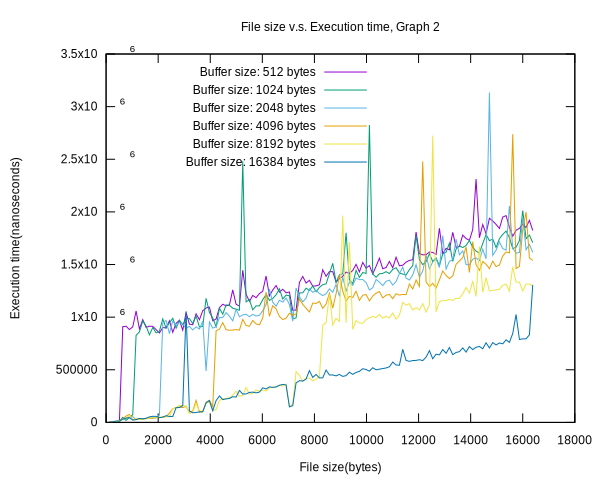
\includegraphics{../png/graph2.png}
\caption{16384 bytes以内の範囲のバッファの書き出しの速度のグラフ}
\end{figure}

図1からバッファなし、バッファありの書き出しではバッファありの書き出しの方が高速であるとわかった。
図1、図2から、バッファのサイズがファイルサイズより大きい範囲では、バッファのサイズとファイルの書き出し速度に相関は見られなかった。また、図2からは、書き出すファイルのサイズがバッファサイズを超えると、書き出しに\(1\times 10^{6}\)付近かそれ以上の実行時間が掛かることがわかった。

\hypertarget{ux8003ux5bdf}{%
\section{考察}\label{ux8003ux5bdf}}

バッファのサイズがファイルサイズより大きい範囲でバッファのサイズとファイルの書き出し速度に相関がないことと、書き出すファイルのサイズがバッファサイズを超えるときに書き出しに\(1\times 10^{6}\)付近かそれ以上の実行時間が掛かることは、共通の背景があると考えられる。

bufio.WriterのWriter関数の実装{[}1{]}から、bufio.Writerのbufの空きがなくなるまで、bufに書き込みを行い、bufの空きがなくなったときにのみ、Flush()関数でbufの中身をメモリに書き込むために、write(2)システムコールを呼び出すことになっている。bufio.Writerによるファイルの書き出しに、write(2)システムコールが呼ばれることは、straceコマンド(Linux)、dtrussコマンド(Mac
OS)で検証できる。write(2)システムコールはユーザー空間のメモリ領域をカーネル空間にあるページキャシュに書き写す処理があるので、そのときにオーバーヘッドが生じる。そのためバッファリングを行って逐一write(2)システムコールの回数を少なくすることで、書き出しの高速化ができるようになる。

また、OSのファイルAPIの観点からでは、Linuxのファイルシステムであるext4では、ブロックといわれる単位でファイル読み書きを扱っていて、そのブロックのサイズが4096
bytes{[}2{]}なので、4096
bytesの自然数倍じゃないバッファサイズで書き込みをすると無駄な切り上げが生じる。なので、実験の結果とファイルAPIの実装の観点から、省メモリを無視した場合、ファイルの書き出しを高速化するには、バッファサイズを4096の自然数倍のバイトでなるべく大きく確保するべきだと考えられる。

\hypertarget{ux53c2ux8003ux6587ux732e}{%
\section{参考文献}\label{ux53c2ux8003ux6587ux732e}}

{[}1{]} Google.''src/bufio/bufio.go''.Google Open Source.2022-05-03.
https://cs.opensource.google/go/go/+/refs/tags/go1.19.4:src/bufio/bufio.go;l=663
,(参照 2023-01-08). {[}2{]} Linus
Torvalds.''fsverity''.GitHub.2022-06-10.
https://github.com/torvalds/linux/blob/master/Documentation/filesystems/fsverity.rst\#ext4
,(参照 2023-01-08).

\end{document}
